%*******************************************************************************
%****************************** Fifth Chapter *********************************
%*******************************************************************************

\chapter{Quantifying Human-Humanoid Imitation Activities} \label{chapter7}
%
%% **************************** Define Graphics Path **************************
%\ifpdf
%    \graphicspath{{chapter7/figs/raster/}{chapter7/figs/PDF/}{chapter7/figs/}}
%\else
%    \graphicspath{{chapter7/figs/vector/}{chapter7/figs/}}
%\fi
\graphicspath{{figs/chapter6/PDF/}}


%
%%**************************** %Broad Purpose  **********************************
%\section*{Summary and broad purpose of the chapter}
%* How long (number of words)?
%* Deadline
%* What have you got?
%


%\section{Human-Humanoid Imitation Activities} 
%\section{Results}\label{sec:results}
\section{Introduction} 

We investigated the robustness and weaknesses of the reconstructed 
state spaces (RRSs) using the uniform time-delay embedding technique (UTDE) 
and recurrence plots (RPs) for recurrent quantification analysis (RQA) 
methodologies in the following conditions: 
\begin{itemize}

\item Three levels of smoothness for the normalised data 
(sg0zmuv, sg1zmuv and sg2zmuv), computed from two different filter 
lengths (29 and 159) with the same polynomial degree of 5 using the 
function \texttt{sgolay(p,n,m)} \cite{Rsignal},

\item Four velocities arm movement activities: horizontal normal (HN), 
	horizontal faster (HF), vertical normal (VN), and 
	vertical faster (VF), and
\item Four window lengths: 2-sec (100 samples), 5-sec (250 samples), 
	10-sec (500 samples) and 15-sec (750 samples).
\end{itemize}

Further details about the prepartions of time series are presented in
Section \ref{sec:preparation_timeseries}.

%It is important to note that after the data collection in the experiment, 
%raw time series were windowed, normalised and smoothed as presented in 


\section{Time series}
To make comparison easier, we only present 10-sec (500 samples) window length 
time series for three participants (p01, p01 and p03) performing horizontal 
arm movements (axis GyroZ) and  vertical arm movements (axis GyroY) 
(Figs \ref{fig:tsH} and \ref{fig:tsV}), other data is then presented in 
Appendix \ref{appendix:d}.
We consider different levels of smoothness of the normalised data 
with two different Savitzky-Golay filter lengths (29 and 159) 
with the same polynomial degree of 5 using \texttt{sgolay(p,n,m)} 
\citep{Rsignal}.
 
%%---------------------------------(FIGURE)-------------------------------------
\begin{figure}[!h]
  \centering
\includegraphics[width=1.0\textwidth]{tsHv03}
    	\caption{ 
	{\bf Time series for horizontal arm movements.}
		(A) raw-normalised (sg0zmuvGyroZ), 
		(B) normalised-smoothed 1 (sg1zmuvGyroZ) and
		(C) normalised-smoothed 2 (sg2zmuvGyroZ).
		Time series are only for three participants (p01, p02, and p03) 
		for horizontal movements in normal and faster velocity (HN, HF) 
		with the normalised GyroZ axis (zmuvGyroZ) 
		and with one sensor attached to the participant (HS01) 
		and other sensor attached to the robot (RS01).	
	R code to reproduce the figure is available from \cite{hwum2018}.
        }
    \label{fig:tsH}
\end{figure}
%%---------------------------------(FIGURE)------------------------------------
%%---------------------------------(FIGURE)-------------------------------------
\begin{figure}[!h]
  \centering
\includegraphics[width=1.0\textwidth]{tsVv03}
	\caption{ 
	{\bf Time series for vertical arm movements.}
		(A) raw-normalised (sg0zmuvGyroY), 
		(B) normalised-smoothed 1 (sg1zmuvGyroY) and
		(C) normalised-smoothed 2 (sg2zmuvGyroY).
		Time series are only for three participants (p01, p02, and p03) 
		for vertical movements in normal and faster velocity (VN, VF) 
		with the normalised GyroY axis (zmuvGyroY) 
		and with one sensor attached to the participant (HS01) 
		and other sensor attached to the robot (RS01).
		R code to reproduce the figure is available 
		from \cite{hwum2018}.
        }
    \label{fig:tsV}
\end{figure}
%%---------------------------------(FIGURE)------------------------------------









\section{Minimum Embedding Parameters}


%\subsection{UTDE for time series in the context of human-robot interaction}
The first step to create RSSs with the use of UTDE is to compute the
average minimum embedding parameters for all participants, sensors and 
activities using False Nearest Neighbour (FNN) and 
Average Mutual Information algorithms (AMI).

Hence, for the average minimum embedding dimension, 
Figs \ref{fig:caoH} and \ref{fig:caoV} show the minimum embedding 
dimension for twenty participants for the horizontal and vertical arm
movements at normal and faster velocity (HN, HF, VN, and VF) with the 
human attached sensor (HS01) and robot attached sensor (RS01).
Generally, Figs \ref{fig:caoH} and \ref{fig:caoV} show that the minimum 
embedding values appear to be more constant for sensor RS01 than the 
slightly variations for embedding values for sensor HS01.
It can also be seen in Figs~\ref{fig:caoH} and \ref{fig:caoV} that there 
is a minor decrease of minimum embedding values as smoothness of time 
series increase. 

%%---------------------------------(FIGURE)-------------------------------------
\begin{figure}[!h]
\centering
\includegraphics[width=1.0\textwidth]{cao_aHw10}
	\caption{
	{\bf Minimum embedding dimensions for horizontal arm movements.} 
		(A, B) Horizontal Normal (HN), (C, D) Horizontal Faster (HF) 
		movements,
		(A, C) sensor attached to participants (HS01), and
		(B, D) sensor attached to robot (RS01).
		Minimum embedding dimensions are for twenty participants 
		(p01 to p20) with three smoothed signals 
		(sg0zmuvGyroZ, sg1zmuvGyroZ and sg2zmuvGyroZ)
		and window lenght of 10-sec (500 samples).
		R code to reproduce the figure is available 
		from \cite{hwum2018}.
        }
    \label{fig:caoH}
\end{figure}
%%---------------------------------(FIGURE)------------------------------------
%%---------------------------------(FIGURE)-------------------------------------
\begin{figure}[!h]
\centering
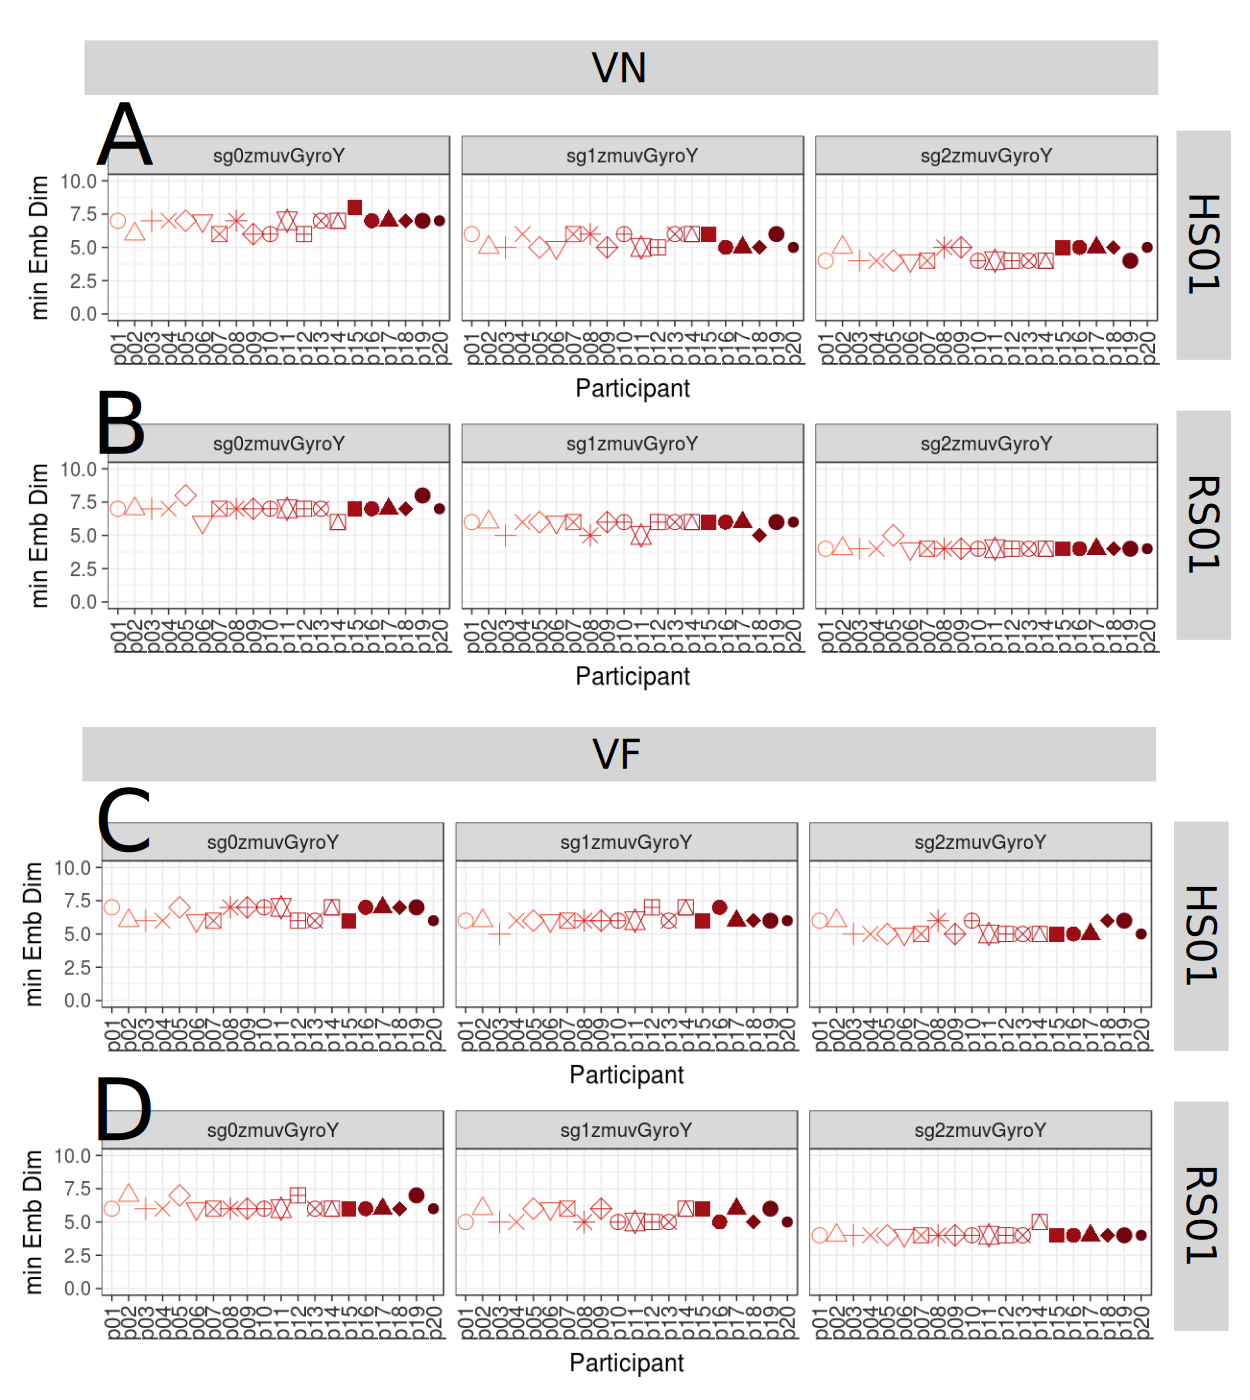
\includegraphics[width=1.0\textwidth]{cao_aVw10}
	\caption{
	{\bf Minimum embedding dimensions for vertical arm movements.} 
		(A, B) Vertical Normal (VN), (C, D) Vertical Faster (VF) 
		movements,
		(A, C) sensor attached to participants (HS01), and		
		(B, D) sensor attached to robot (RS01).
		Minimum embedding dimensions are for twenty participants 
		(p01 to p20) with three smoothed signals (sg0zmuvGyroY, 
		sg1zmuvGyroY and sg2zmuvGyroY) 
		and window length of 10-sec (500 samples).
		R code to reproduce the figure is available 
		from \cite{hwum2018}.
        }
    \label{fig:caoV}
\end{figure}
%%---------------------------------(FIGURE)------------------------------------

Similarly, the first minimum values of the Average Mutual Information (AMI) 
for participants (p01-p20), activities (HN, HF, VN, and VF) and 
sensors (HS01, RS01) is shown in Figs~\ref{fig:amiH} and \ref{fig:amiV}.
Hence, Fig~\ref{fig:amiH}(A) shows that the first minimum values of AMI,
for normal horizontal arm movements, tend to be more spread as the smoothness 
of the time series is increasing while AMI values for faster horizontal arm 
movements in Fig~\ref{fig:amiH}(C) show little effect with regards
to its fluctuation as the smoothness of time series increase.
Fig~\ref{fig:amiH}(B) shows that minimum values of AMI are 
less spread as smoothness is increasig. However, values for horizontal
faster movements in Fig~\ref{fig:amiH}(D) tend to be more spread as 
smoothness is increasing.
%the high frequencies on robots movements in the horizontal normal movement.
With regard to vertical arm movements,
the minimum values of AMI in Figs~\ref{fig:amiV}(A) and ~\ref{fig:amiV}(C) 
show a slightly increase of the spread values as the smoothness is increasing
and minimum AMI values in Fig~\ref{fig:amiV}(B) appear to have less 
fluctuations as the smoothness of the time series is increasing, however, 
that do not happen for the second smoothed values (sg2zmuvGyroY) in 
Fig~\ref{fig:amiV}(D) which appear to be constant.
It can be noted that the increase of fluctuations of minimum AMI values 
in Figs~\ref{fig:amiH} and \ref{fig:amiV} is due to the smoothed curves in 
the AMIs as the smoothness of time series is increasing.

%%---------------------------------(FIGURE)-------------------------------------
\begin{figure}[!h]
\centering
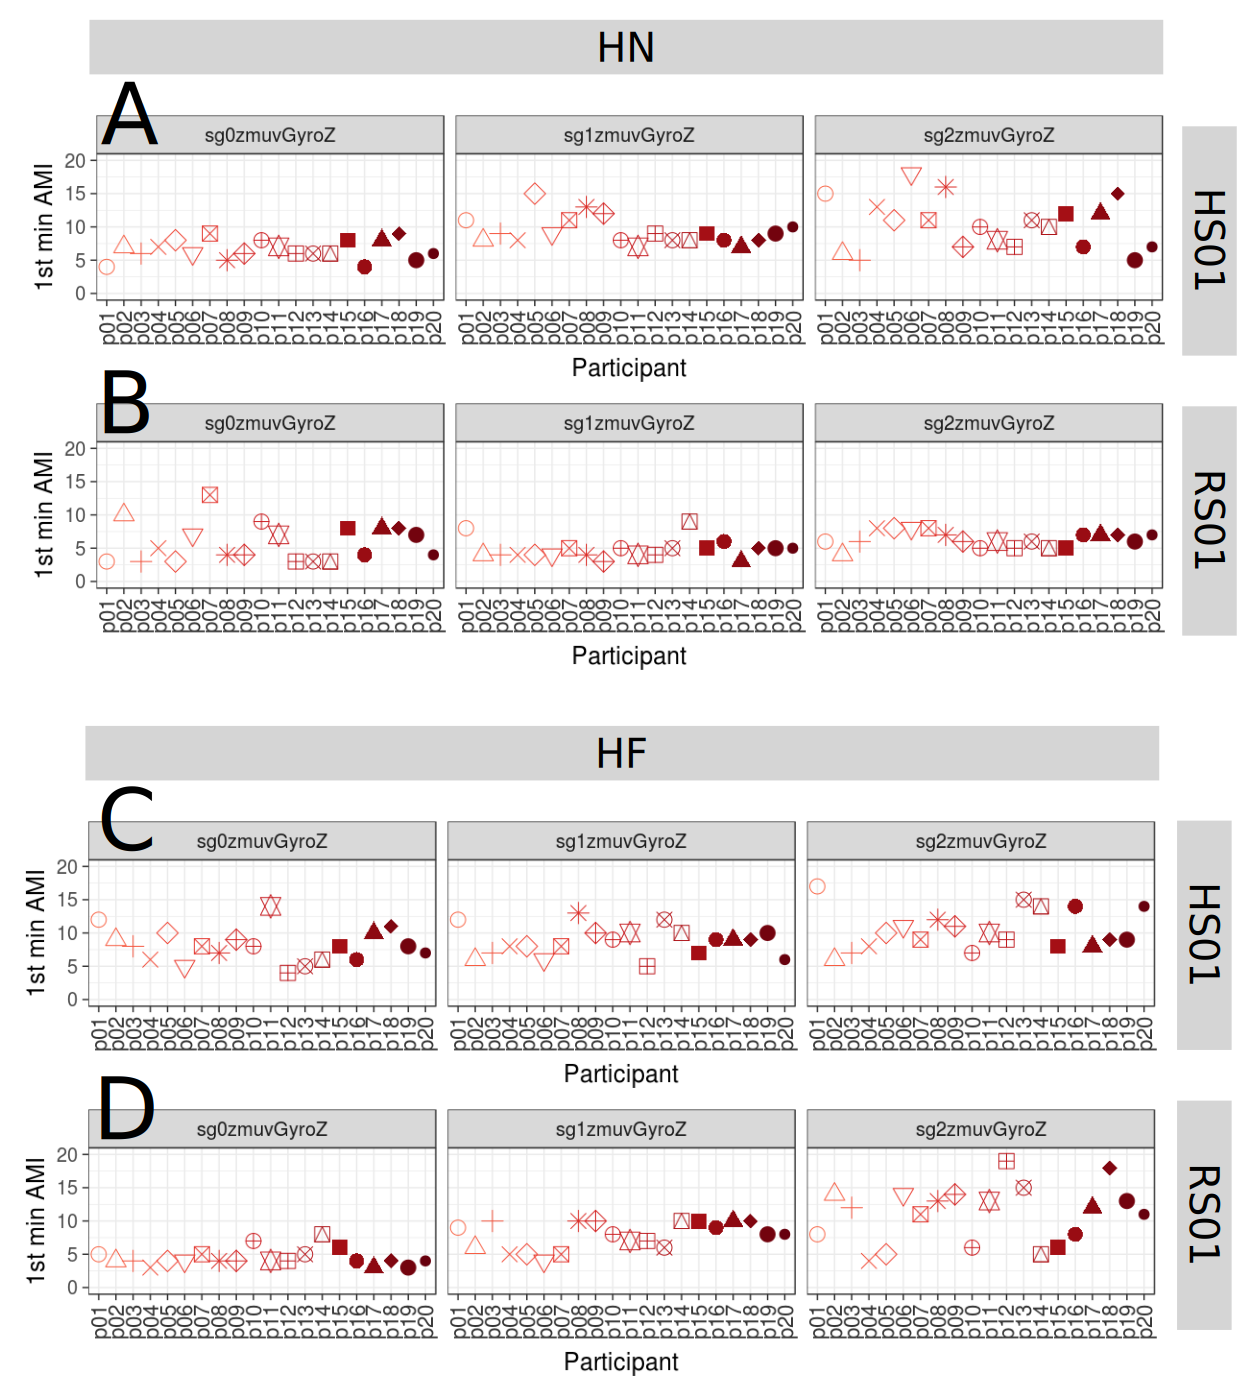
\includegraphics[width=1.0\textwidth]{ami_aHw10}
	\caption{
	{\bf First minimum AMI values for horizontal arm movements.}
		(A, B) Horizontal Normal (HN), (C, D) Horizontal Faster (HF) 
		movements,
		(A, C) sensor attached to participants (HS01), and
		(B, D) sensor attached to robot (RS01).
		First minimum AMI values are for twenty participants 
		(p01 to p20) with three smoothed signals (sg0zmuvGyroZ, 
		sg1zmuvGyroZ and sg2zmuvGyroZ) and  window lenght of 
		10-sec (500 samples).
		R code to reproduce the figure is available 
		from \cite{hwum2018}.
        }
    \label{fig:amiH}
\end{figure}
%%---------------------------------(FIGURE)------------------------------------
%%---------------------------------(FIGURE)-------------------------------------
\begin{figure}[!h]
\centering
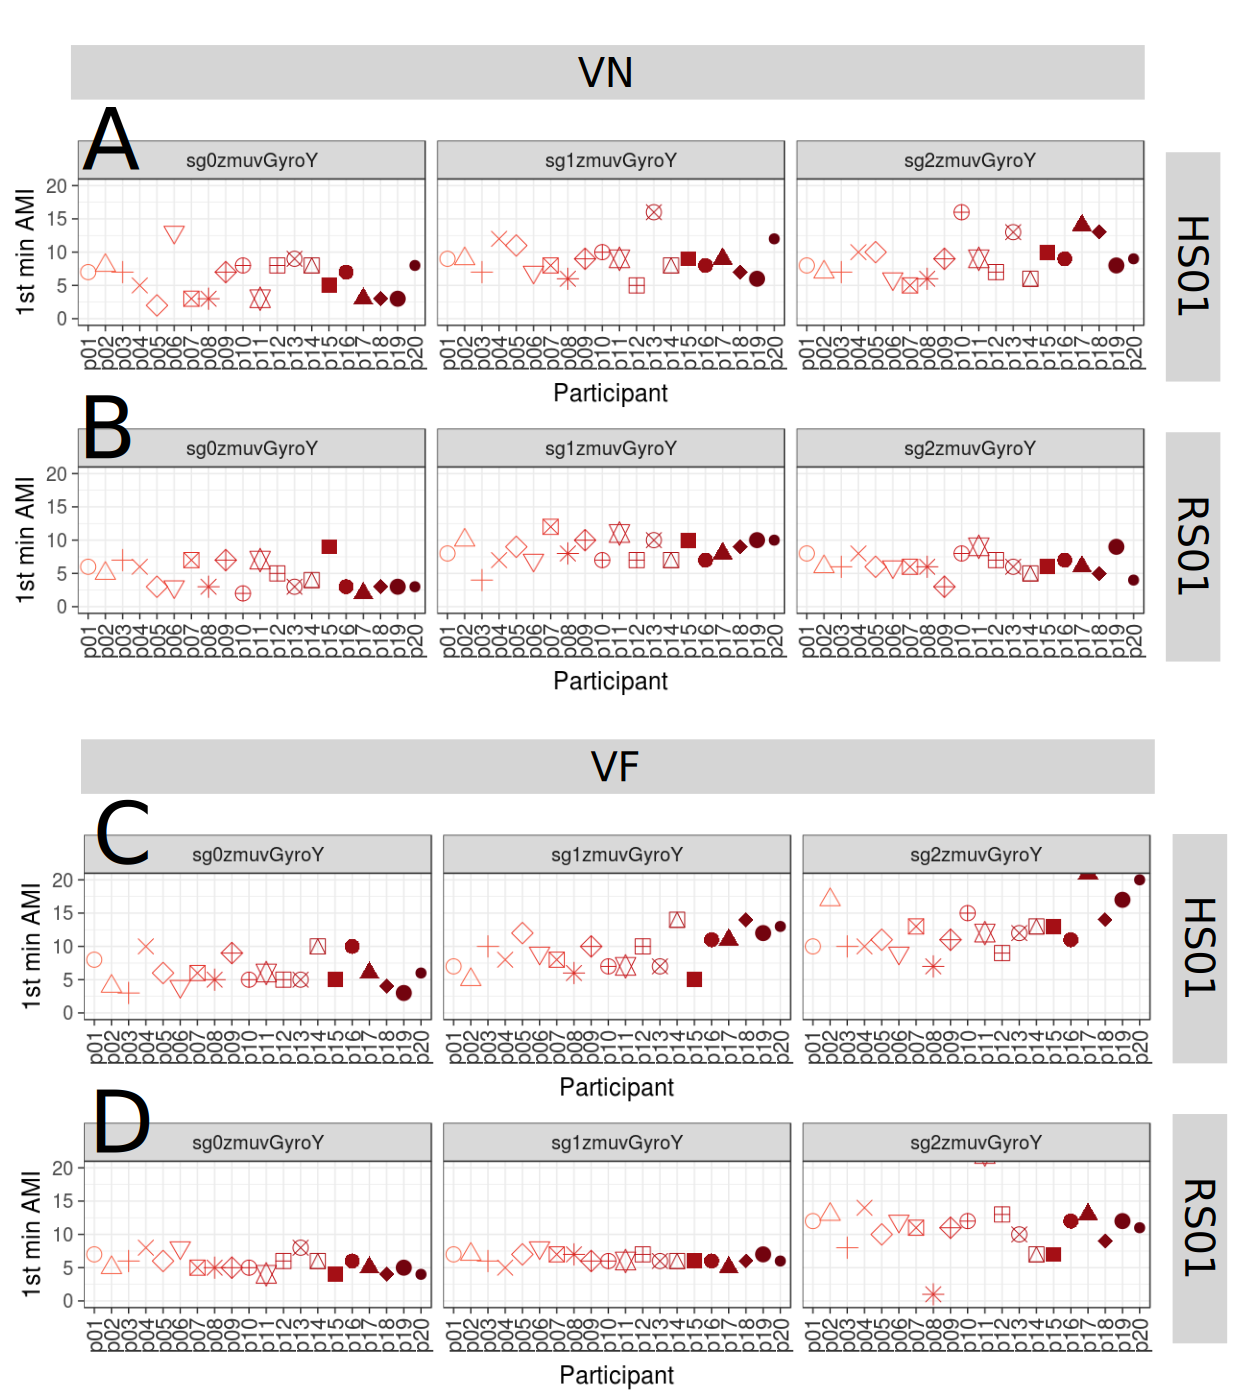
\includegraphics[width=1.0\textwidth]{ami_aVw10}
	\caption{
	{\bf First minimum AMI values for vertical arm movements.}
		(A, B) Vertical Normal (VN), (C, D) Vertical Faster (VF) 
		movements,
		(A, C) sensor attached to participants (HS01), and
		(B, D) sensor attached to robot (RS01).
		First minimum AMI values are for twenty participants 
		(p01 to p20) with three smoothed signals (sg0zmuvGyroZ, 
		sg1zmuvGyroZ and sg2zmuvGyroZ) and  window lenght of 
		10-sec (500 samples).
		R code to reproduce the figure is available 
		from \cite{hwum2018}.
        }
    \label{fig:amiV}
\end{figure}
%%---------------------------------(FIGURE)------------------------------------



\section{Reconstructed state spaces with UTDE}
Although the implementation of Uniform Time-Delay Embedding matrix (UTDE) 
is simple, the main challenge in this regard is to select embedding parameters 
to reconstruct the state spaces for each time series, considering that time 
series are unique in terms of its structure (modulation of amplitude, 
frequency and phase) \citep{ frank2010, sama2013, bradley2015}.
With that in mind, the problem is not to compute individual embedding parameters 
for each of the time series but to deal with the selection of two parameters 
that can represent all the time series. 
Our solution for that problem was, therefore, to compute a sample mean over 
all values that represents all participants, sensors and activities 
(Section \ref{sec:overall_minMT}).
Hence, the sample mean for the minimum values of $E_{1}(m)$ from 
Figs~\ref{fig:caoH} and \ref{fig:caoV} is $\overline{m}_0=6$ and the sample 
mean for minimum values of AMIs from Figs~\ref{fig:amiH} and \ref{fig:amiV} 
is $\overline{\tau}_0=8$, for which the average minimum embedding parameters 
is ($\overline{m_0}=6$, $\overline{\tau_0}=8$).

Therefore, considering time series for participant 01 
(Figs \ref{fig:tsH}, \ref{fig:tsV}) the reconstructed state spaces
for horizontal arm movements (Figs~\ref{fig:rss_aHw10}) and
 vertical arm movements  (Figs~\ref{fig:rss_aVw10}) 
are computed with $\overline{m_0}=6$ and $\overline{\tau_0}=8$ 
(Section \ref{sec:rsswithUTDE}).
%%---------------------------------(FIGURE)-------------------------------------
\begin{figure}[!h]
\centering
\includegraphics[height=0.85\textheight]{rss_aH}
\caption{
	{\bf RSSs for horizontal arm movements.}
	Reconstructed state spaces %for time series of Figure \ref{fig:tsH}.
	of participant p01 for horizontal movements in normal and faster 
	velocity (HN, HF) with raw-normalised (sg0zmuvGyroZ), 
	normalised-smoothed 1 (sg1zmuvGyroZ) and 
	normalised-smoothed 2 (sg2zmuvGyroZ) time series of the 
	sensors attached to the participant (HS01) and other sensor 
	attached to the robot (RS01).	
	Reconstructed state spaces were computed with 
	embedding parameters $m=6$, $\tau=8$.
	R code to reproduce the figure is available from \cite{hwum2018}.
        }
    \label{fig:rss_aHw10}
\end{figure}
%%---------------------------------(FIGURE)------------------------------------
%%---------------------------------(FIGURE)-------------------------------------
\begin{figure}[!h]
\centering
\includegraphics[height=0.85\textheight]{rss_aV}
    \caption{
	{\bf RSSs for vertical arm movements.}
	Reconstructed state spaces %for time series of Figure \ref{fig:tsV}.
	of participant p01 for vertical movements in normal and faster 
	velocity (VN, VF) with raw-normalised (sg0zmuvGyroZ), 
	normalised-smoothed 1 (sg1zmuvGyroZ) and 
	normalised-smoothed 2 (sg2zmuvGyroZ) time series of the 
	sensors attached to the participant (HS01) and other sensor 
	attached to the robot (RS01).	
	Reconstructed state spaces were computed with 
	embedding parameters $m=6$, $\tau=8$.
	R code to reproduce the figure is available from \cite{hwum2018}.
        }
    \label{fig:rss_aVw10}
\end{figure}
%%---------------------------------(FIGURE)------------------------------------


The RSSs for horizontal normal and faster from the human sensors (HS01)
are slightly smoothed as the time-series smoothness increase
Figs~\ref{fig:rss_aHw10}(A,C). Similarly, the smoothness of RSSs 
for robot sensor (RS01) is smoothed as the time series smoothness increase.
Although the frequency of the movement increase from normal to faster velocity, 
the RSSs in Figs~\ref{fig:rss_aHw10}(B)
show highers osciallations specially for a maximum values of smoothnes,
while the RSS for HF in Figs~\ref{fig:rss_aHw10}(D) show a lower and smothed
osicallations as the smoothenss increase.


Although time series for vertical movements are less noisy and well structured
(Figs \ref{fig:tsV}), the RSSs (Figs \ref{fig:rss_aVw10}) seems to be less 
organised, specially for Fig \ref{fig:rss_aVw10}(A,C), while time series 
for vertical faster movements (VF) having more periods (Figs \ref{fig:tsV})
create RSS with well defined patters (\ref{fig:rss_aVw10}(C,D)).
It is important to note that smoothness of time series creates also an effect
on smoothness in the trajectories of the RSS being the RS01 more organised
and more persistent while trajectories for HS01 are more changeable.

Therefore, one can observe by eye the differences in each of the trajectories 
in the reconstructed state spaces 
(Figs~\ref{fig:rss_aHw10}, \ref{fig:rss_aVw10}), 
however one might be not objective when quantifying 
those differences since such observations might vary from person to person.
With that in mind, in our early experiments, we tried to objectively 
quantify those differences using euclidean distances between the origin 
to each of the points in the trajectories in RSSs, however these created 
suspicious metrics, specially for trajectories which looked very messy.
Hence, we take advantage of the Recurrence Quantification Analyses
in order to objectively quantify the differences in each of the cases 
of the time series.


%\subsection{RPs and RQA for time series in the context of 
%human-robot interaction}

\section{Recurrences Plots}
Considering the time series of Figs~\ref{fig:tsH} and \ref{fig:tsV}, 
we computed its Recurrence Plots for horizontal arm movements 
(Fig~\ref{fig:rp_aH}) and vertical arm movements (Fig~\ref{fig:rp_aV}) 
using the average embedding parameters ($m=6$, $\tau=8$) and a recurrence 
threshold of $\epsilon=1$. Regarding the selection of recurrence threshold,
Marwan et al. \cite{marwan2011} pointed out that choosing an appropriate 
recurrence threshold is crucial to get meaningful representations in RPs, 
however, for our work where quantifying movement variability is our aim,
we give little importance to the selection of the recurrence threshold as
as long as it is able to represent the dynamical transitions in each of the 
time series.


Generally, the increase of smoothness in time series results in ticker 
and more well defined diagonal lines in the RPs 
Regarding the low and hight frequencies in the time series due to the 
changes in velocities of the movements, RPs patterns
show both an increase of diagonal lines and a decrease of its thickness.
Although, RPs patterns show consistency with the movements type and velocities,
it can be noticed that RPs for HS01 are not entirely well defined
while RPs for RS01 shown a more consistent pattern
(Fig~\ref{fig:rp_aV}, \ref{fig:rp_aH}). 
%One can see in Figs~\ref{fig:rp_aH}(A,B) thats
%Fig~\ref{fig:rp_aV}, \ref{fig:rp_aH}

It is important to note that only RPs for participant 01 are presented
in (Fig~\ref{fig:rp_aV}, \ref{fig:rp_aH}), however
RPs for other participants are in Appendix \ref{appendix:d:rps} in which 
it can also visualised slightly similar patterns in the RPs.
With that in mind, we can highlight that, as similar as, the 
Reconstructed State Spaces (Figs~\ref{fig:rss_aHw10}, \ref{fig:rss_aVw10}), 
the patterns in the RPs can be easily noticed by eye for different conditions 
of the time series (Figs~\ref{fig:rp_aH}, Fig~\ref{fig:rp_aV}),
which lead us to apply Recurrence Quantification Analysis 
in order to have a more objective quantification for the movement 
variability for each of the conditions of the time series.

%%---------------------------------(FIGURE)-------------------------------------
\begin{figure}[!h]
\centering
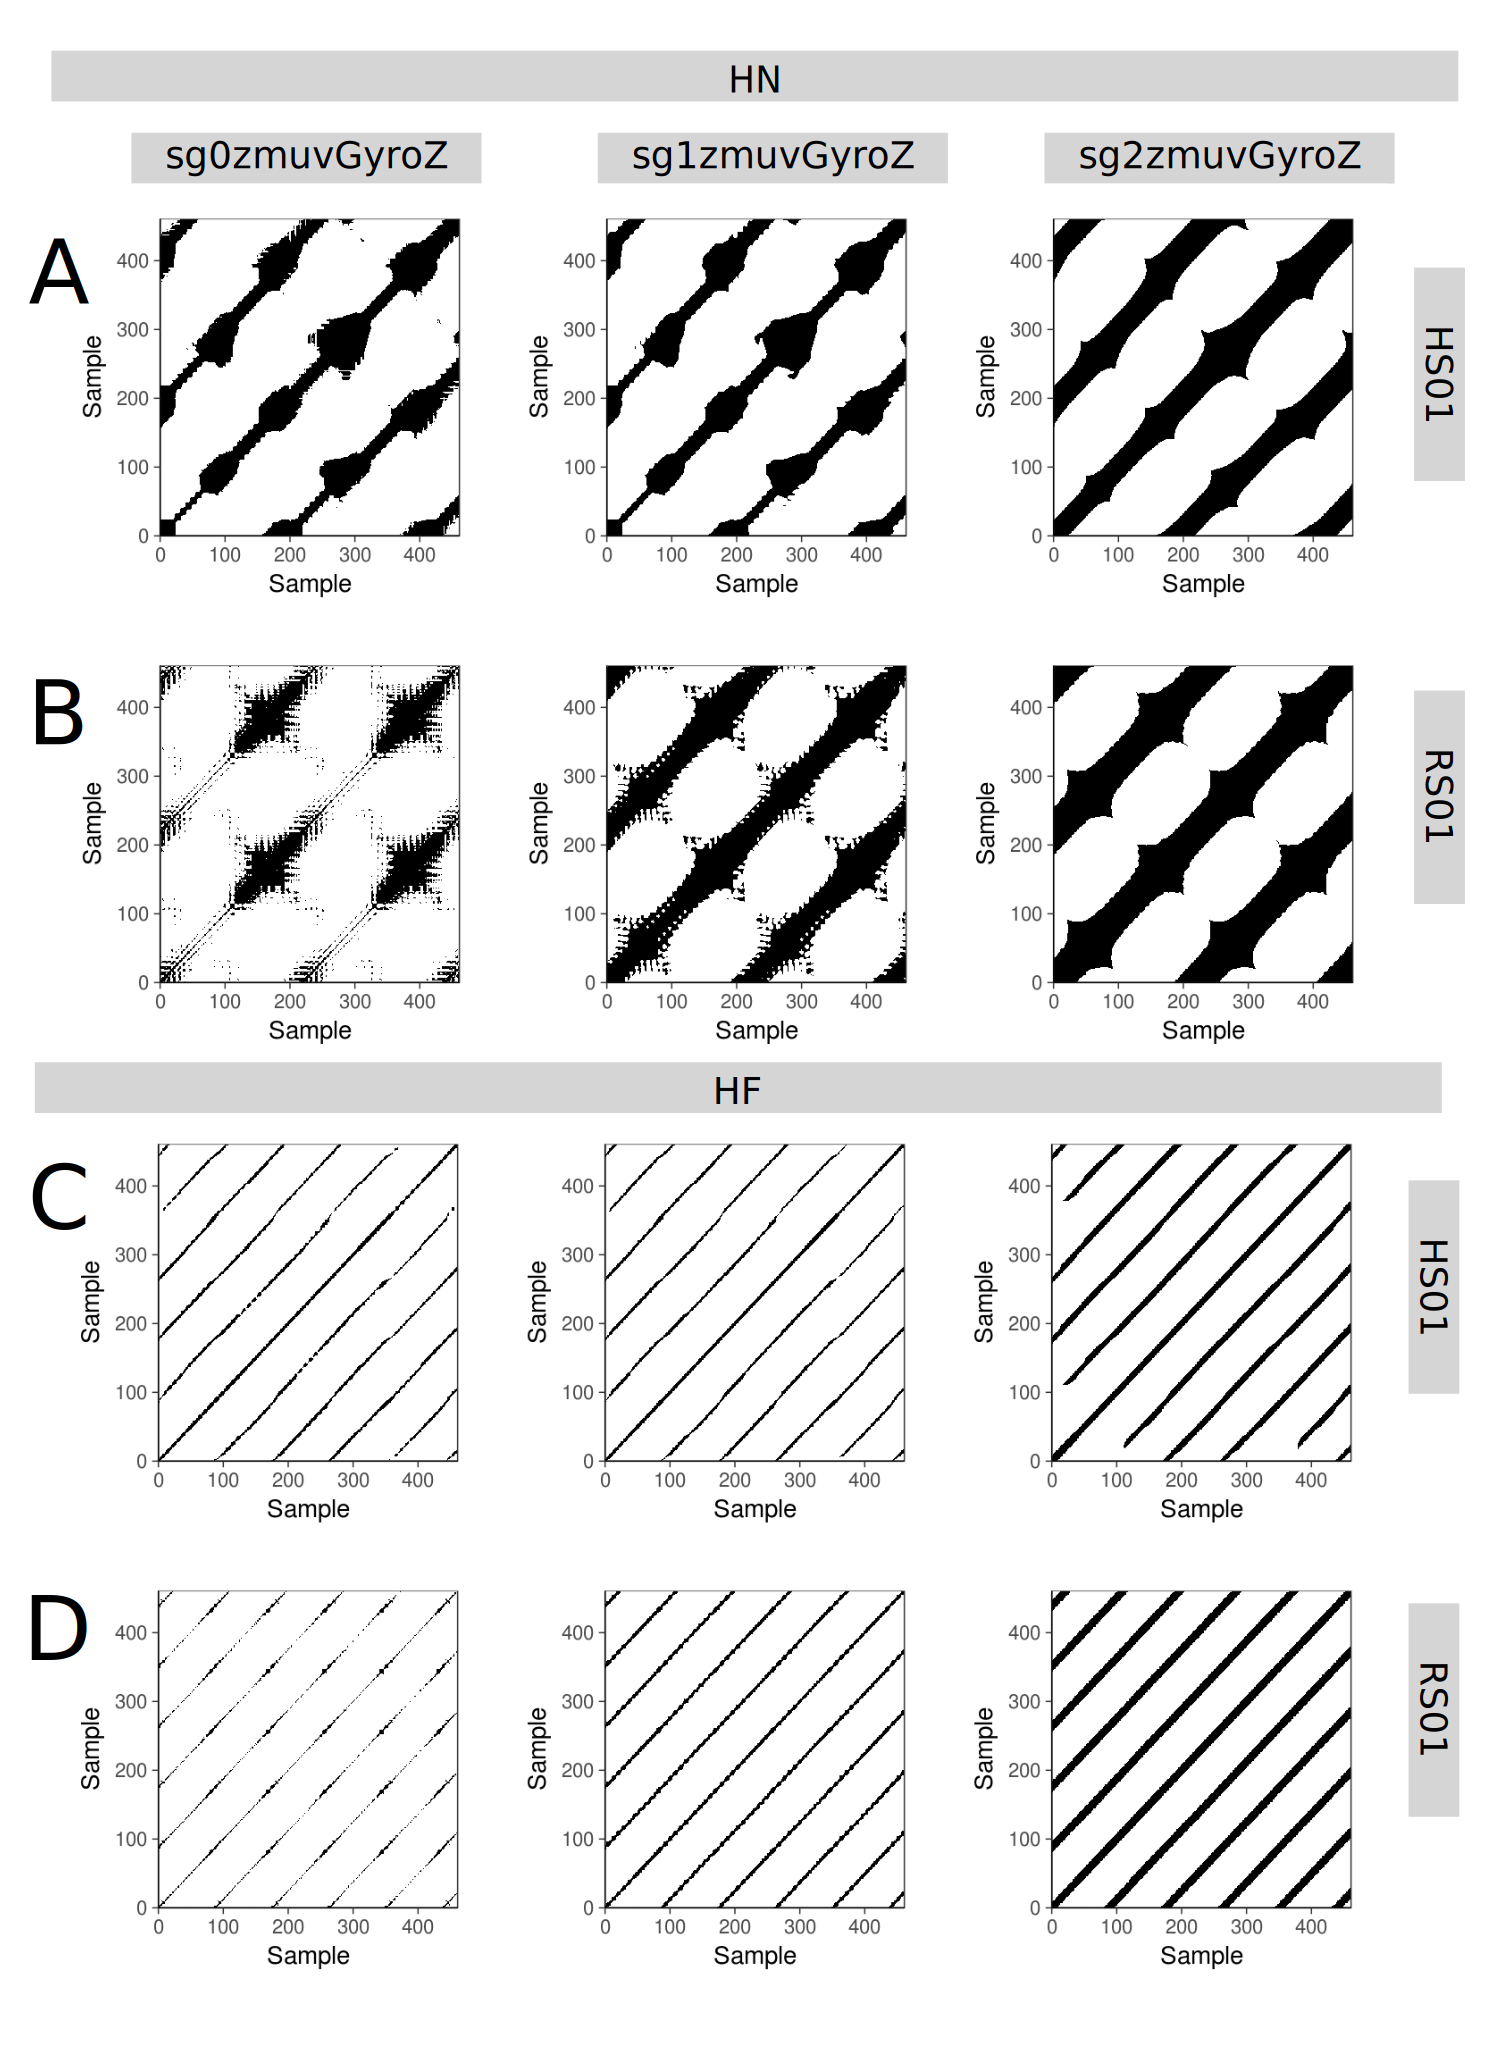
\includegraphics[height=0.85\textheight]{rp_aH}
\caption{
	{\bf RPs for horizontal arm movements.}	
	Recurrence plots %for time series of Figure \ref{fig:tsV}.
	of participant p01 for horizontal movements in normal and faster 
	velocity (HN, HF) with raw-normalised (sg0zmuvGyroZ), 
	normalised-smoothed 1 (sg1zmuvGyroZ) and 
	normalised-smoothed 2 (sg2zmuvGyroZ) time series of the 
	sensors attached to the participant (HS01) and other sensor 
	attached to the robot (RS01).
	Recurrence plots were computed with 
	embedding parameters $m=6$, $\tau=8$ and $\epsilon=1$.
	R code to reproduce the figure is available from \cite{hwum2018}.
        }
    \label{fig:rp_aH}
\end{figure}
%%---------------------------------(FIGURE)------------------------------------
%%---------------------------------(FIGURE)-------------------------------------
\begin{figure}[!h]
\centering
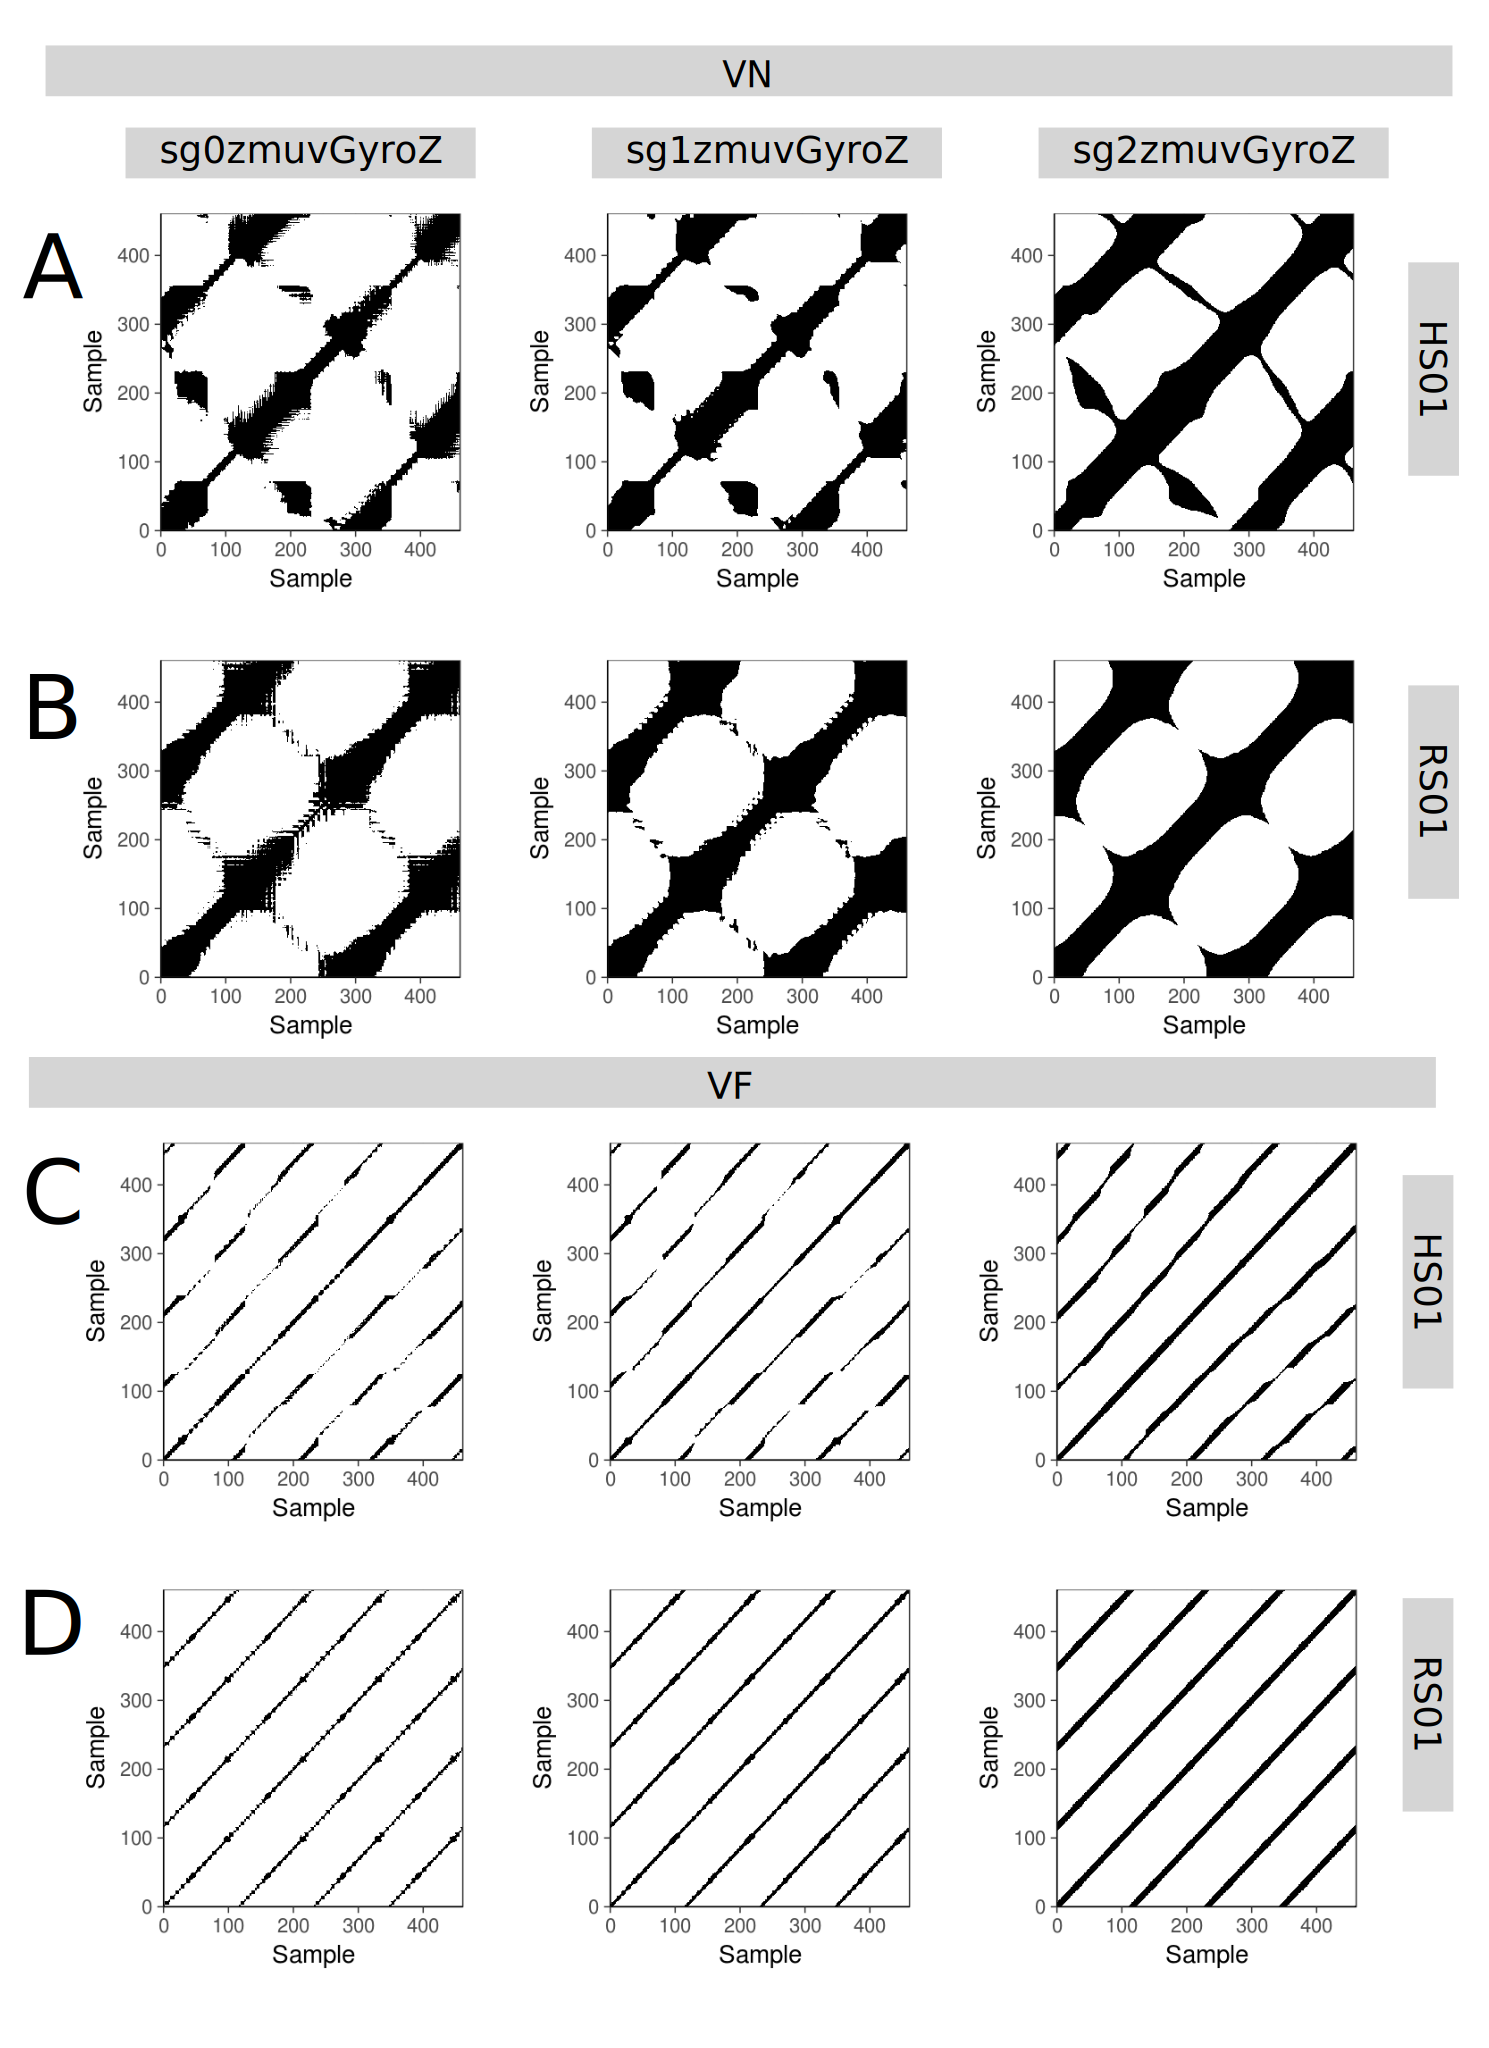
\includegraphics[height=0.85\textheight]{rp_aV}
\caption{
	{\bf RPs for vertical arm movements.}	
	Recurrence plots %for time series of Figure \ref{fig:tsV}.
	of participant p01 for vertical movements in normal and faster 
	velocity (VN, VF) with raw-normalised (sg0zmuvGyroZ), 
	normalised-smoothed 1 (sg1zmuvGyroZ) and 
	normalised-smoothed 2 (sg2zmuvGyroZ) time series of the 
	sensors attached to the participant (HS01) and other sensor 
	attached to the robot (RS01).
	Recurrence plots were computed with 
	embedding parameters $m=6$, $\tau=8$ and $\epsilon=1$.
	R code to reproduce the figure is available from \cite{hwum2018}.
        }
    \label{fig:rp_aV}
\end{figure}
%%---------------------------------(FIGURE)------------------------------------






\section{Recurrence Quantification Analysis}

Considering the RPs for 20 participants performing HN, HF, VN and VF
with the sensor attached to the human HS01 and the humanoid robot RS01 
and with the increase of smoothness 
(sg0zmuvGyroZ, sg1zmuvGyroZ and sg2zmuvGyroZ), 
four metrics of RQA metrics (REC, DET, RATIO and ENTR) 
are computed with embedding parameters $m=6$, $\tau=8$ and $\epsilon=1$
in the following subsections.



%RPs provided pattern formations for each of the time series 
%conditions (Figs~\ref{fig:rp_aH} and \ref{fig:rp_aV}).

\subsection{REC values}
In Figs~\ref{fig:rec_aH} and \ref{fig:rec_aV} can be seen that REC values 
are more spread for HN than HF movements with data coming from HS01 sensor. 
In contrast, REC values appear to be constant and present 
little variation for both HN and HF movements 
with data from the sensor attached to the humanoid robot RS01.
With regard to the increase of smoothness of data (sg0zmuvGyroZ, sg1zmuvGyroZ and sg2zmuvGyroZ), 
REC values present little variation as the smoothness is increasing for data 
from HS01 and REC values more similar as the smoothness is increasing for data from RS01.
%%---------------------------------(FIGURE)-------------------------------------
\begin{figure}[!h]
\centering
\includegraphics[width=1.0\textwidth]{rec_aH}
    \caption{
	{\bf REC values for horizontal arm movements.}	
	REC values (representing \% of black dots in the RPs) for 
	20 participants performing HN and HF movements
	with sensors HS01, RS01 and three smoothed-normalised axis 
	of GyroZ (sg0zmuvGyroZ, sg1zmuvGyroZ and sg2zmuvGyroZ).
	REC values were computed with 
	embedding parameters $m=6$, $\tau=8$ and $\epsilon=1$
	R code to reproduce the figure is available from \cite{hwum2018}.
        }
    \label{fig:rec_aH}
\end{figure}
%%---------------------------------(FIGURE)------------------------------------
%%---------------------------------(FIGURE)-------------------------------------
\begin{figure}[!h]
\centering
\includegraphics[width=1.0\textwidth]{rec_aV}
    \caption{
	{\bf REC values for vertical arm movements.}	
	REC values (representing \% of black dots in the RPs) for 
	20 participants performing VN and VF movements
	with sensors HS01, RS01 and three smoothed-normalised axis 
	of GyroY (sg0zmuvGyroY, sg1zmuvGyroY and sg2zmuvGyroY).
	REC values were computed with 
	embedding parameters $m=6$, $\tau=8$ and $\epsilon=1$.
	R code to reproduce the figure is available from \cite{hwum2018}.
        }
    \label{fig:rec_aV}
\end{figure}
%%---------------------------------(FIGURE)------------------------------------







\subsection{DET values}
Little can be said with regard to the variation of DET values
as these change very little even for type of movement or type of sensor
(Figs~\ref{fig:det_aH} and \ref{fig:det_aV}).
With regard to the smoothness of time series, DET values appear to be more similar 
as the smoothness of the data is increasing.
%%---------------------------------(FIGURE)-------------------------------------
\begin{figure}[!h]
\centering
\includegraphics[width=1.0\textwidth]{det_aH}
    \caption{
	{\bf DET values for horizontal arm movements.}	
    	DET values (representing predictability and organisation of the RPs) for 
	20 participants performing HN and HF movements
	with sensors HS01, RS01 and three smoothed-normalised axis 
	of GyroZ (sg0zmuvGyroZ, sg1zmuvGyroZ and sg2zmuvGyroZ).
	DET values were computed with 
	embedding parameters $m=6$, $\tau=8$ and $\epsilon=1$.
	R code to reproduce the figure is available from \cite{hwum2018}.
        }
    \label{fig:det_aH}
\end{figure}
%%---------------------------------(FIGURE)------------------------------------
%%---------------------------------(FIGURE)-------------------------------------
\begin{figure}[!h]
\centering
\includegraphics[width=1.0\textwidth]{det_aV}
    \caption{
	{\bf DET values for vertical arm movements.}	
    	DET values (representing predictability and organisation of the RPs) for 
	20 participants performing VN and VF movements
	with sensors HS01, RS01 and three smoothed-normalised axis 
	of GyroY (sg0zmuvGyroY, sg1zmuvGyroY and sg2zmuvGyroY).
	DET values were computed with 
	embedding parameters $m=6$, $\tau=8$ and $\epsilon=1$.
	R code to reproduce the figure is available from \cite{hwum2018}.
        }
    \label{fig:det_aV}
\end{figure}
%%---------------------------------(FIGURE)------------------------------------







\subsection{RATIO values}
RATIO values for HN movements vary less than HF movements for HS01 sensor 
which is similar behaviour of RATIO values for RS01 sensors 
in both vertical and horizontal movements (Figs~\ref{fig:ratio_aH} and \ref{fig:ratio_aV}).
It can also noticed a decrease of variation in RATIO values as the smoothness of the signal is increasing.
%%---------------------------------(FIGURE)-------------------------------------
\begin{figure}[!h]
\centering
\includegraphics[width=1.0\textwidth]{ratio_aH}
    \caption{
	{\bf RATIO values for horizontal arm movements.}
	RATIO (representing dynamic transitions) for 
	20 participants performing HN and HF movements
	with sensors HS01, RS01 and three smoothed-normalised axis 
	of GyroZ (sg0zmuvGyroZ, sg1zmuvGyroZ and sg2zmuvGyroZ).
	RATIO values were computed with 
	embedding parameters $m=6$, $\tau=8$ and $\epsilon=1$.
	R code to reproduce the figure is available from \cite{hwum2018}.
        }
    \label{fig:ratio_aH}
\end{figure}
%%---------------------------------(FIGURE)------------------------------------
%%---------------------------------(FIGURE)-------------------------------------
\begin{figure}[!h]
\centering
\includegraphics[width=1.0\textwidth]{ratio_aV}
    \caption{
	{\bf RATIO values for vertical arm movements.}
	RATIO (representing dynamic transitions) for 
	20 participants performing VN and VF movements
	with sensors HS01, RS01 and three smoothed-normalised axis 
	of GyroY (sg0zmuvGyroY, sg1zmuvGyroY and sg2zmuvGyroY).
	RATIO values were computed with
	embedding parameters $m=6$, $\tau=8$ and $\epsilon=1$.
	R code to reproduce the figure is available from \cite{hwum2018}.
        }
    \label{fig:ratio_aV}
\end{figure}
%%---------------------------------(FIGURE)------------------------------------


\subsection{ENTR values}
ENTR values show more variation for HS01 sensor than ENTR values for RS01 sensor
which appear to be more constant and the smoothness of data affects little 
to the variation of ENTR values (Figs~\ref{fig:entr_aH} and \ref{fig:entr_aV}).
%%---------------------------------(FIGURE)-------------------------------------
\begin{figure}[!h]
\centering
\includegraphics[width=1.0\textwidth]{entr_aH}
    \caption{
	{\bf ENTR values for horizontal arm movements.}
    	ENTR values (representing the complexity of the deterministic structure in time series) for 
	20 participants performing HN and HF movements
	with sensors HS01, RS01 and three smoothed-normalised axis 
	of GyroZ (sg0zmuvGyroZ, sg1zmuvGyroZ and sg2zmuvGyroZ).
	ENTR values were computed with 
	embedding parameters $m=6$, $\tau=8$ and $\epsilon=1$.
	R code to reproduce the figure is available from \cite{hwum2018}.
        }
    \label{fig:entr_aH}
\end{figure}
%%---------------------------------(FIGURE)------------------------------------
%%---------------------------------(FIGURE)-------------------------------------
\begin{figure}[!h]
\centering
\includegraphics[width=1.0\textwidth]{entr_aV}
    \caption{
	{\bf ENTR values for vertical arm movements.}
    	ENTR values (representing the complexity of the deterministic structure in time series) for 
	20 participants performing VN and VF movements
	with sensors HS01, RS01 and three smoothed-normalised axis 
	of GyroY (sg0zmuvGyroY, sg1zmuvGyroY and sg2zmuvGyroY).
	ENTR values were computed with 
	embedding parameters $m=6$, $\tau=8$ and $\epsilon=1$.
	R code to reproduce the figure is available from \cite{hwum2018}.
        }
    \label{fig:entr_aV}
\end{figure}
%%---------------------------------(FIGURE)------------------------------------



%
%
%%% \subsection{Effects of different parameters in the computation of different metrics of RQA.}
%%Then we only select the axis AccY and GyroZ as being the axis which show 
%%better consistency in the patters for all the posibilities int he time series.
%%That was doing visual inspection. It also worthwhile to note that those axis
%%represent the majoy energy amothn other axis for both sensors.
%%The selection of recurrecne threshold is 1 for HF activites,
%%however this should be changed to
%%for HN activies.
%%With that we also can observe the effect of the seletion 
%%of recurrence threshold for different actibities is crucial 
%%to have meaninign values in the metrics of RQA.
%%% added: Tue 19 Jun 2018
%
%
%
%
%
%
%\subsection{RQA metrics with different embedding parameters, recurrence thresholds, 
%window lengths, levels of smoothness, and time series structures.}
%Zbilut et al. \cite{zbilut1992} established RQA metrics with the aim of determining 
%embedding parameters, their method consisted on creating 3D surfaces with RQA metrics 
%with an increase of embedding parameters ($m$ and $\tau$), then 
%Zbilut et al. \cite{zbilut1992} explored fluctuations and gradual changes in the 3D surfaces
%that provide information about the embeddings.
%Much recently, Marwan et al. \cite{marwan2015} created 3D surfaces for visual selection 
%of not only embedding parameters but also recurrence thresholds. 
%Following same methodologies, we explored the stability and robustness of RQA metrics (REC, DET, RATIO and ENTR)
%using 3D surfaces by an unitary increase of the pair embedding parameters ($0 \ge m \le 10$, $0 \ge \tau \le 10$) 
%and a decimal increase of 0.1 for recurrence thresholds ($ 0.2 \ge \epsilon \le 3 $) (Fig.~\ref{fig:topo_rqas}).
%We also computed 3D surfaces of RQA metrics for different sensors and different activities (Fig.~\ref{fig:topo_sensoractivities}).
%RQA metrics are also affected by the window length where for example four 
%window lengths of 100, 250, 500 and 750 samples (Fig.~\ref{fig:topo_windows}).
%Three level of smoothness were computed for RQA metrics showing 
%smoothed 3D surfaces ad the level of smoothness increase (Fig.~\ref{fig:topo_smoothness}).
%Similarly, 3D surfaces of RQA metrics were also computed for three participants (Fig.~\ref{fig:topo_participants}).
%%%---------------------------------(FIGURE)-------------------------------------
%\begin{figure}[!ht]
%\centering
%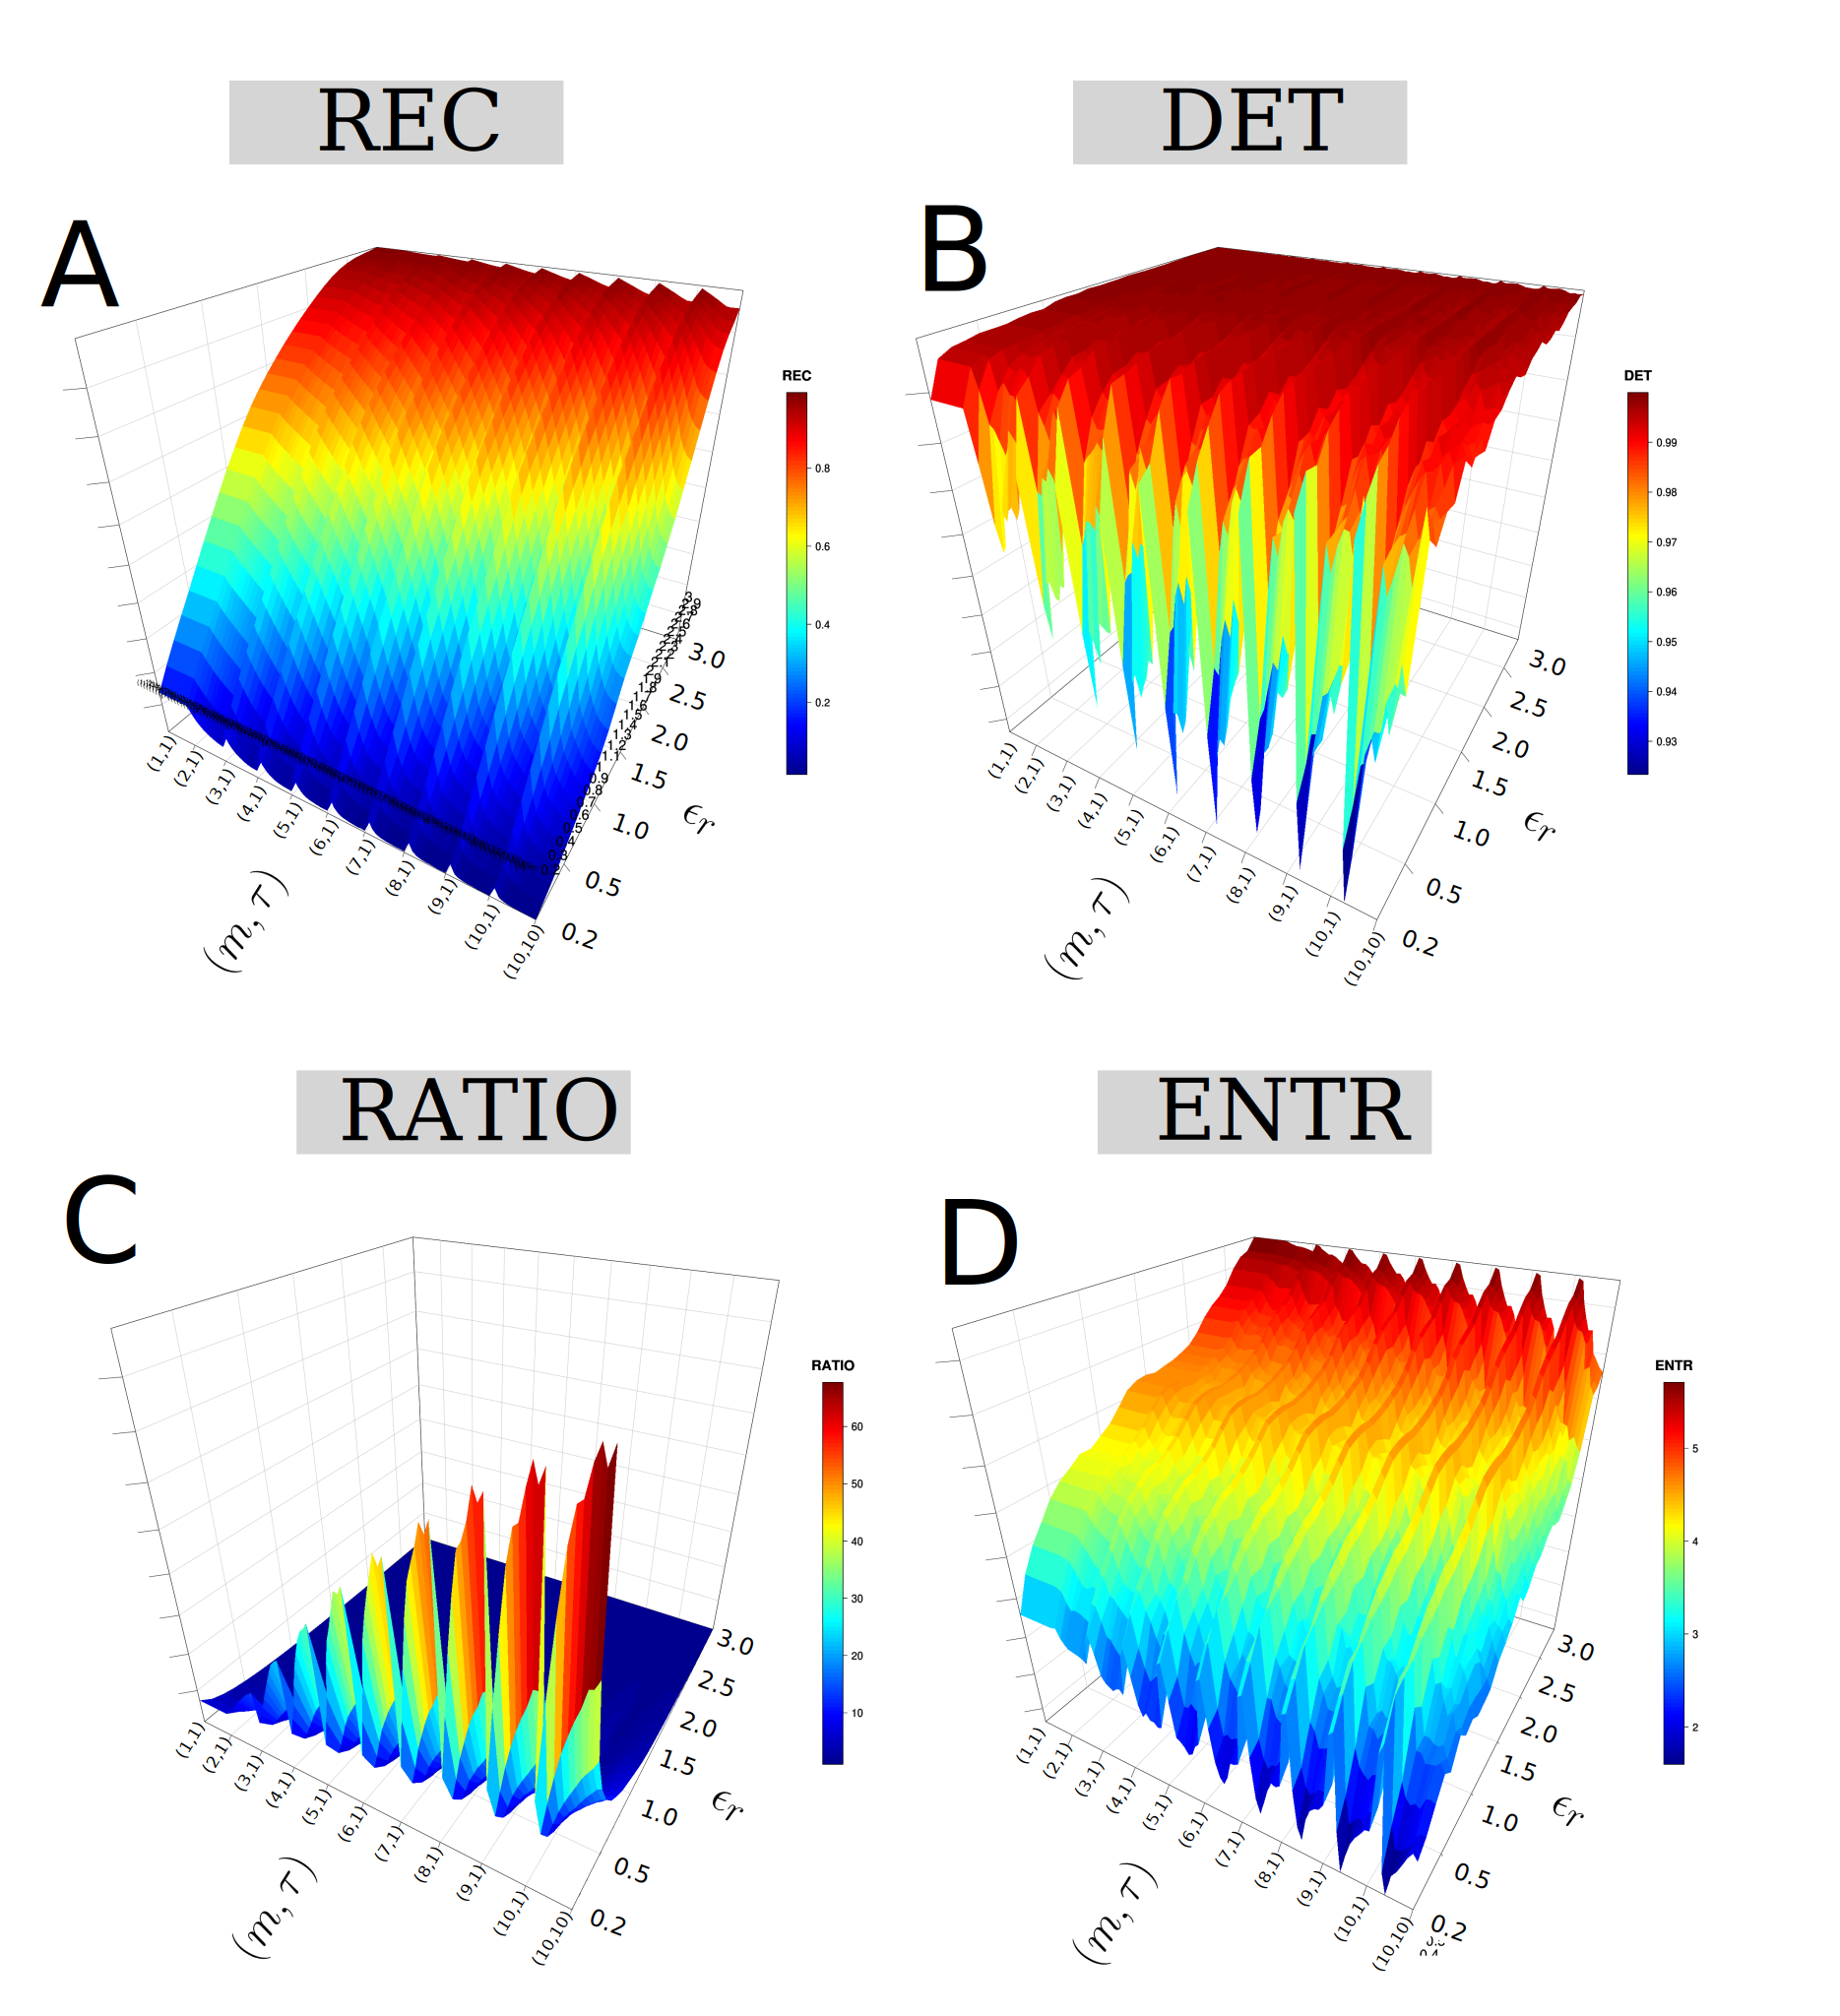
\includegraphics[width=1.0\textwidth]{rqas}
%    \caption{
%	{\bf 3D surfaces for RQA metrics.}
%	3D surfaces for REC, DET, RATIO and ENTR values with increasing 
%	pair embedding parameters ($0 \ge m \le 10$, $0 \ge \tau \le 10$) 
%	and recurrence thresholds (  $ 0.2 \ge \epsilon \le 3 $).
%	RQA metrics values for time series of participant p01 using HS01 sensor, 
%	HN activity and sg0zmuvGyroZ axis and 500 samples window length.
%        R code to reproduce the figure is available from \cite{hwum2018}.
%	}
%\label{fig:topo_rqas}
%\end{figure}
%%%---------------------------------(FIGURE)------------------------------------
%%%---------------------------------(FIGURE)-------------------------------------
%\begin{figure}[!ht]
%\centering
%\includegraphics[width=1.0\textwidth]{sa}
%    \caption{
%	{\bf 3D surfaces of RQA metrics for sensors and activities.}
%	3D surfaces with increasing embedding parameters and recurrence thresholds are 
%	for HS01 and RS01 sensors of HN, HF, VN and VF activities.
%	RQA metrics values are for time series of participant p01 for sensors (HS01 and RS01), 
%	activities (HN, HF, VN and VF) and for 	sg0zmuvGyroZ axis  with 500 samples window length. 
%	R code to reproduce the figure is available from \cite{hwum2018}.
%       }
%\label{fig:topo_sensoractivities}
%\end{figure}
%%%---------------------------------(FIGURE)-------------------------------------
%%%---------------------------------(FIGURE)-------------------------------------
%\begin{figure}[!ht]
%\centering
%\includegraphics[width=1.0\textwidth]{w}
%    \caption{
%	{\bf 3D surfaces for RQAs metrics with four window lengths.}
%	3D surfaces of RQAs metric values with increasing embedding parameters and recurrence thresholds 
%	are for four window lengths (w100, w250, w500 and  w750).
%	RQA metrics values are for time series of participant p01 
%	using HS01 sensor, HN activity and sg0zmuvGyroZ axis.
%	R code to reproduce the figure is available from \cite{hwum2018}.
%        }
%\label{fig:topo_windows}
%\end{figure}
%%%---------------------------------(FIGURE)------------------------------------
%%%---------------------------------(FIGURE)-------------------------------------
%\begin{figure}[!ht]
%\centering
%\includegraphics[width=1.0\textwidth]{s}
%    \caption{
%	{\bf 3D surfaces for RQA metrics with three levels of smoothness.}
%       	3D surfaces of RQAs metric values with increasing embedding parameters and recurrence thresholds 
%	are for three levels of smoothness (sg0zmuvGyroZ, sg1zmuvGyroZ and sg1zmuvGyroZ).
%	RQA metrics values are for time series of participant p01 using HS01 sensor, 
%	HN activity and 500 samples window length.
%	R code to reproduce the figure is available from \cite{hwum2018}.
% }
%\label{fig:topo_smoothness}
%\end{figure}
%%%---------------------------------(FIGURE)------------------------------------
%
%
%%%---------------------------------(FIGURE)-------------------------------------
%\begin{figure}[!ht]
%\centering
%\includegraphics[width=1.0\textwidth]{p}
%    \caption{
%	{\bf 3D surfaces for RQA metrics with three participants.}
%       	3D surfaces of RQAs metric values for participants p01, p02 and p03 
%	with increasing embedding parameters and recurrence thresholds.
%	RQA metrics values are for time series of HS01 sensor, 
%	HN activity and 500 samples window length.
%	R code to reproduce the figure is available from \cite{hwum2018}.
% }
%\label{fig:topo_participants}
%\end{figure}
%%%---------------------------------(FIGURE)------------------------------------
%
%
%
%




